\chapter{Fase I: la decisión de la Primera Línea vista desde 2013}\label{cap:evaluacion2013}

Este capítulo aplica el modelo de los \cref{cap:modelo,cap:simulacion,cap:optimizacion} con las
condiciones de 2013. Primero se recalibra la red al año 2013 y se construyen los escenarios de demanda
que un planificador de entonces habría considerado razonables. Luego se evalúan, con esa información,
las alternativas de primera línea (evaluación \emph{ex ante}) y, por último, se repite la evaluación
con la trayectoria de demanda que efectivamente ocurrió (evaluación \emph{ex post}).

\section{El modelo con las condiciones de 2013}

\paragraph{Red y calibración.} Se conserva la estructura de la red de la fase II (zonas, corredores,
funciones de congestión y parámetro gravitacional) y se retiran los proyectos posteriores a 2013. La
demanda de hora pico del año base es de \ViajesPicoDosMilTrece{} mil viajes motorizados, obtenida de
la Encuesta de Movilidad 2011 \citep{sdm2012}, y la población de Bogotá se fija en las proyecciones
de entonces. Se recalibran dos parámetros, la escala de capacidad vial y la constante modal del
transporte público, para reproducir la velocidad vial de hora pico (\VelDosMilTrece{} km/h) y la
participación del transporte público entre motorizados (\PartTPDosMilTrece). El ajuste es exacto: la
escala de capacidad resulta de \EscalaDosMilTrece{} vehículos por hora, la constante modal de
\ASCDosMilTrece{} minutos, el hacinamiento máximo de \HacDosMilTrece{} y la duración media del viaje,
que no se calibra, de \TiempoDosMilTrece{} minutos.

\paragraph{Escenarios vistos desde 2013.} Las derivas de la demanda se toman de lo que se esperaba
entonces: las zonas de Bogotá crecen en promedio 1,27\,\% anual, como en las proyecciones del censo de
2005, con las mismas diferencias entre zonas que en la fase II; los municipios de la región crecen
3\,\% anual; la tendencia común de los viajes por persona es de 1\,\% anual y la volatilidad la misma
de la fase II. Se simulan \NFaseUno{} escenarios con la misma técnica (Sobol aleatorizado y solución
exacta del MBG) entre 2013 y 2050.

\paragraph{Alternativas.} La \cref{tab:alternativas2013} resume las alternativas evaluadas. Todos los
costos están en billones de pesos de 2025: provienen del estudio de la Empresa Metro de 2023 en pesos
de noviembre de 2022 \citep{emb2023} y se indexan con la inflación de 2023 a 2025 (factor
\Indexacion). El costo oficial del subterráneo corresponde al diseño de 2014--2015; el costo con
unitarios aplica a esa misma línea los costos por kilómetro y por estación del estudio de 2023, que
reflejan precios de una concesión real (\cref{sec:costos_metro}). Las dos tipologías reciben la misma
distribución lognormal de sobrecostos, con media de 44,7\,\% \citep{flyvbjerg2005wb}; si los túneles
tienen más riesgo de sobrecosto que los viaductos, como sugiere la experiencia internacional, este
supuesto favorece al subterráneo.

\begin{table}[ht]
\centering\small
\caption{Alternativas de primera línea en la evaluación de 2013.}\label{tab:alternativas2013}
\begin{tabular}{p{4.6cm}rrrrrr}
\toprule
Alternativa & km & Est. & Capacidad & Vel. & Obra & CAPEX \\
 & & & pas/h-sentido & km/h & años & billones \\
\midrule
Elevado Bosa--calle 72 & 23,96 & 16 & 72.000 & 43 & 5 & \CapexElevadoLuno \\
Subterráneo Américas--calle 127 (costo oficial) & 27 & 27--28 & 80.000 & 36 & 7 & \CapexSubOficial \\
Subterráneo (costo con unitarios de 2023) & 27 & 28 & 80.000 & 36 & 7 & \CapexSubUnitarios \\
\bottomrule
\end{tabular}
\fuente{CONPES 3900 \citep{conpes3900}; diseño de 2014 \citep{fdn2015}; estudio EMB \citep{emb2023};
cálculos del autor. CAPEX base, sin sobrecostos.}
\end{table}

En la evaluación central ambas obras empiezan en 2016, tras los estudios: el elevado abre en 2021 y el
subterráneo, que tarda dos años más en construirse, en 2023. Como el diseño de 2014 preveía abrir el
subterráneo en 2021 \citep{fdn2015}, se evalúa también esa variante, que con siete años de obra exige
empezar en 2014 y, por tanto, gastar antes. El valor presente se calcula a 2014 con la tasa de 12\,\% vigente entonces y, como
sensibilidad, con 9\,\% y 6,4\,\%.

\section{Evaluación \emph{ex ante}}

La \cref{tab:fase2013} y la \cref{fig:fase2013_beneficios} presentan el beneficio neto de cada
alternativa frente a no construir metro.

\begin{table}[ht]
\centering\small
\caption{Evaluación \emph{ex ante} de la primera línea con la información de 2013: CAPEX esperado con
sobrecostos y beneficio neto esperado frente a no construir metro (billones de pesos de 2025, valor
presente a 2014).}\label{tab:fase2013}
\resizebox{\textwidth}{!}{\begin{tabular}{p{5.2cm}rrrrrr}
\toprule
Diseño (visto desde 2013) & CAPEX & \multicolumn{3}{c}{E[BN] a la tasa} & P(BN$>$0) & $\bar t_{2030}$ \\
\cmidrule(lr){3-5}
 & medio & 6,4\,\% & 9\,\% & 12\,\% & al 12\,\% & min \\
\midrule
Elevado \textbar{} $\theta$=0 & 30,6 & 32,6 & 15,5 & 4,6 & 75\,\% & 83,0 \\
Subterráneo (costo oficial) \textbar{} $\theta$=0 & 43,2 & 36,0 & 14,1 & 1,1 & 58\,\% & 80,4 \\
Subterráneo (costo unitarios) \textbar{} $\theta$=0 & 72,6 & 11,8 & -7,2 & -17,4 & 7\,\% & 80,4 \\
Sin metro \textbar{} $\theta$=1 & 0,0 & 52,8 & 34,0 & 21,6 & 100\,\% & 86,8 \\
Elevado \textbar{} $\theta$=1 & 30,6 & 78,4 & 44,2 & 22,4 & 97\,\% & 77,6 \\
Subterráneo (costo oficial) \textbar{} $\theta$=1 & 43,2 & 81,1 & 42,6 & 18,9 & 94\,\% & 75,4 \\
Subterráneo (costo unitarios) \textbar{} $\theta$=1 & 72,6 & 56,9 & 21,3 & 0,4 & 55\,\% & 75,4 \\
Subterráneo (costo oficial, apertura 2021) \textbar{} $\theta$=0 & 43,2 & 38,3 & 14,2 & -0,8 & 49\,\% & 80,4 \\
\bottomrule
\end{tabular}
}
\end{table}

\begin{figure}[ht]
\centering
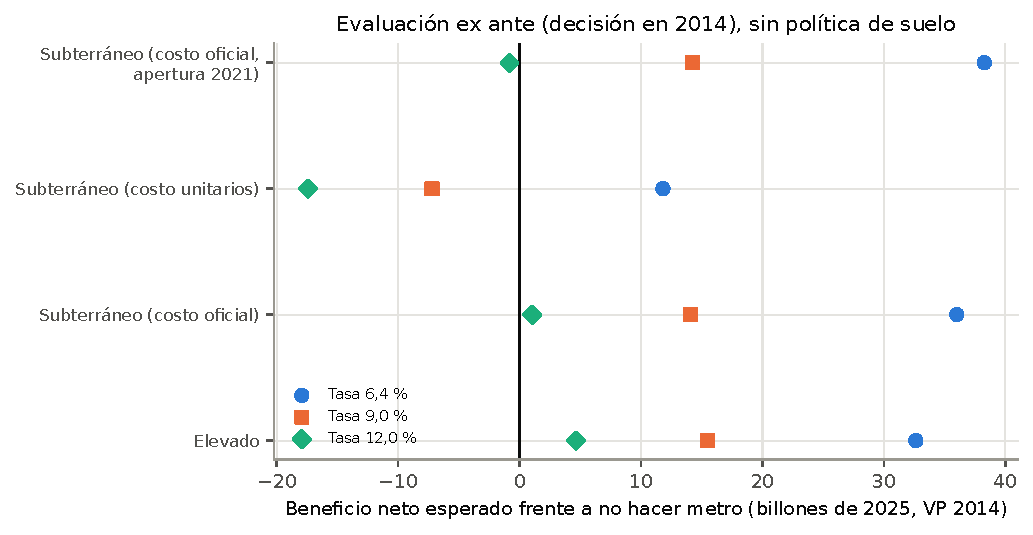
\includegraphics[width=.92\textwidth]{figuras/fig_fase2013_beneficios.pdf}
\caption{Beneficio neto esperado de cada alternativa según la tasa de descuento (evaluación \emph{ex
ante}, sin política de suelo).}\label{fig:fase2013_beneficios}
\end{figure}

\paragraph{Con la tasa de 12\,\%, el metro elevado era la mejor alternativa.} Su beneficio neto
esperado es de \BNElevDoce{} billones, positivo en el \PBNElevDoce{} de los escenarios. El subterráneo
con su costo oficial apenas supera a no construir (\BNSubOfDoce{} billones, \PBNSubOfDoce{} de
probabilidad de ser positivo), y con los costos unitarios de 2023 destruye valor (\BNSubUnDoce{}
billones). Abrir el subterráneo en 2021 no lo mejora a esta tasa (\BNSubOfVeintiunoDoce{} billones):
los años adicionales de beneficios no compensan adelantar el gasto cuando el dinero se descuenta al
12\,\%.

\paragraph{El orden depende de la tasa de descuento.} Con 9\,\% el elevado y el subterráneo de costo
oficial casi empatan (\BNElevNueve{} y \BNSubOfNueve{} billones; \BNSubOfVeintiunoNueve{} si el
subterráneo hubiera abierto en 2021), y con 6,4\,\% el subterráneo de costo oficial supera al elevado
(\BNSubOfSeis{} frente a \BNElevSeis, y \BNSubOfVeintiunoSeis{} con apertura en 2021). La razón es la misma que en la fase II: el subterráneo cuesta
más al principio y entrega más beneficios después, porque llega a la calle 127 y tiene más
estaciones. Con los costos unitarios de 2023, en cambio, el subterráneo queda por debajo del elevado a
todas las tasas.

\paragraph{La política de suelo vuelve a ser la decisión más valiosa.} Por sí sola, la política de
proximidad ($\theta=1$) tiene un beneficio neto esperado de \BNSinMetroTheta{} billones a la tasa de
12\,\%, mayor que el de cualquier metro sin ella; combinada con el elevado llega a \BNElevTheta{}
billones y con el subterráneo de costo oficial a \BNSubOfTheta.

\paragraph{El costo urbano del viaducto.} La comparación anterior no incluye el principal argumento a
favor del subterráneo: el viaducto impone un costo al entorno urbano (ruido, sombra, efecto barrera,
pérdida de valor de los predios vecinos) que el modelo de transporte no ve. La pregunta relevante es
entonces cuánto tendría que valer ese costo para que el subterráneo fuera preferible. Con la tasa de
12\,\%, el costo urbano anual del viaducto que iguala ambas tipologías es de \UmbralOfDoce{} billones
por año con el costo oficial del subterráneo (\UmbralOfVeintiunoDoce{} si abría en 2021) y de
\UmbralUnDoce{} con los costos unitarios; con 9\,\%, de \UmbralOfNueve{} y \UmbralUnNueve{}
respectivamente. El \cref{cap:metro} estima ese costo y discute el resultado.

\section{Evaluación \emph{ex post}}

\paragraph{La demanda fue mucho menor de lo esperado.} La \cref{fig:fase2013_abanico} compara el
abanico de escenarios visto desde 2013 con una trayectoria estilizada de lo ocurrido: crecimiento
moderado hasta 2019, el choque de la pandemia en 2020 y una recuperación incompleta, coherente con la
caída de los viajes entre las encuestas de 2019 y 2023 y con la demanda de TransMilenio
\citep{sdm2024,silla2026}. En 2019 la trayectoria observada ya estaba en el percentil
\PercentilObsPrepandemia{} de los escenarios de 2013, por la menor población; en 2025 está en el
percentil \PercentilObsFin. Un planificador de 2013 que hubiera simulado miles de futuros habría
considerado improbable el que ocurrió. Ese es un argumento para no confiar en un único escenario y,
también, para dar más peso a la cola de baja demanda en decisiones irreversibles.

\begin{figure}[ht]
\centering
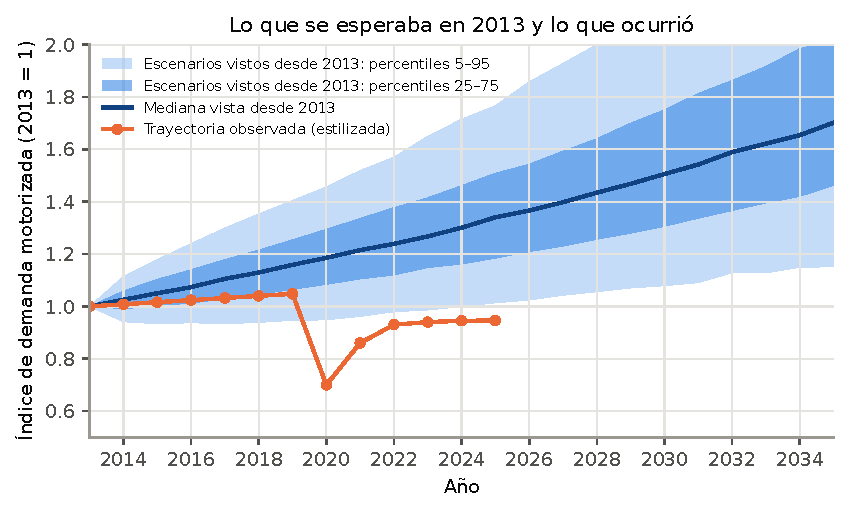
\includegraphics[width=.92\textwidth]{figuras/fig_fase2013_abanico.pdf}
\caption{Índice de demanda motorizada: escenarios vistos desde 2013 y trayectoria observada
estilizada.}\label{fig:fase2013_abanico}
\end{figure}

\paragraph{Con la demanda observada, ninguna primera línea se paga a 12\,\%.} Para la evaluación
\emph{ex post} se usa la trayectoria observada entre 2013 y 2025 y, desde 2026, los escenarios de la
fase II; el valor presente sigue calculándose a 2014 con 12\,\%
(\cref{tab:expost}). El elevado con su apertura real en 2028 tiene un beneficio neto esperado de
\BNExpostElevReal{} billones frente a no haber construido metro. Habría sido peor abrirlo en 2021
(\BNExpostElevDosMilVeintiuno), porque el gasto se habría hecho antes y los años de baja demanda
habrían coincidido con la operación. El subterráneo de costo oficial habría sido peor que el elevado
con cualquier fecha de apertura: \BNExpostSubDosMilVeinticuatro{} billones si abría en 2024,
\BNExpostSubDosMilVeintisiete{} en 2027 y \BNExpostSubDosMilTreinta{} en 2030; con los costos unitarios,
\BNExpostSubUnDosMilVeintisiete.

\begin{table}[ht]
\centering\small
\caption{Evaluación \emph{ex post}: beneficio neto frente a no haber construido metro con la demanda
observada hasta 2025 y los escenarios de la fase II desde 2026 (tasa de 12\,\%, VP a
2014).}\label{tab:expost}
\begin{tabular}{p{6.2cm}rrrrr}
\toprule
Alternativa (año de apertura) & CAPEX & E[BN] & e.e. & P(BN$>$0) & $\bar t_{2030}$ \\
 & \multicolumn{3}{c}{billones COP de 2025} & & min \\
\midrule
Elevado (apertura real 2028) & 30,6 & -4,1 & 0,11 & 12,5\,\% & 50,3 \\
Elevado (si se hubiera decidido en 2014, 2021) & 30,6 & -12,1 & 0,18 & 0,8\,\% & 50,3 \\
Subterráneo oficial (2024) & 43,2 & -15,4 & 0,20 & 0,6\,\% & 49,8 \\
Subterráneo oficial (2027) & 43,2 & -10,2 & 0,16 & 1,6\,\% & 49,8 \\
Subterráneo oficial (2030) & 43,2 & -6,6 & 0,12 & 3,6\,\% & 49,8 \\
Subterráneo unitarios (2027) & 72,6 & -21,8 & 0,24 & 0,0\,\% & 49,8 \\
\bottomrule
\end{tabular}

\end{table}

Estas cifras deben leerse con dos cautelas. La primera es que la red de la fase I no incluye la
troncal de la avenida 68 ni el Regiotram de Occidente, de modo que la evaluación aísla la primera
línea. La segunda es que la tasa de 12\,\% penaliza mucho a cualquier metro; con la tasa actual de
9\,\% y un horizonte más largo los valores mejoran, como muestra la fase II. Lo que el ejercicio
\emph{ex post} sí permite afirmar es que la secuencia de hechos que la ciudad no podía conocer en 2013
(menos población, la pandemia, el retraso) castigó más a la alternativa más costosa.
